\chapter{Interfacing IR sensors}
\label{ch:ir-sensors}
%------------------------------------------------

\ac{IR} stands for Infrared Radiation, is an \ac{EMR} with wavelengths longer than those of visible light. Discovered in 1800 by astronomer Sir William Herschel, \ac{IR} is a region of the \ac{EMR} spectrum where wavelengths range from about 700 nanometers (nm) to 1 millimeter (mm). They are longer than those of visible light, but shorter than those of radio waves. As they do not fall under the visible spectrum, they remain invisible to human eye. Certain animals and cameras can pick up those radiation and perceive them as images.

\begin{figure}
    \centering
	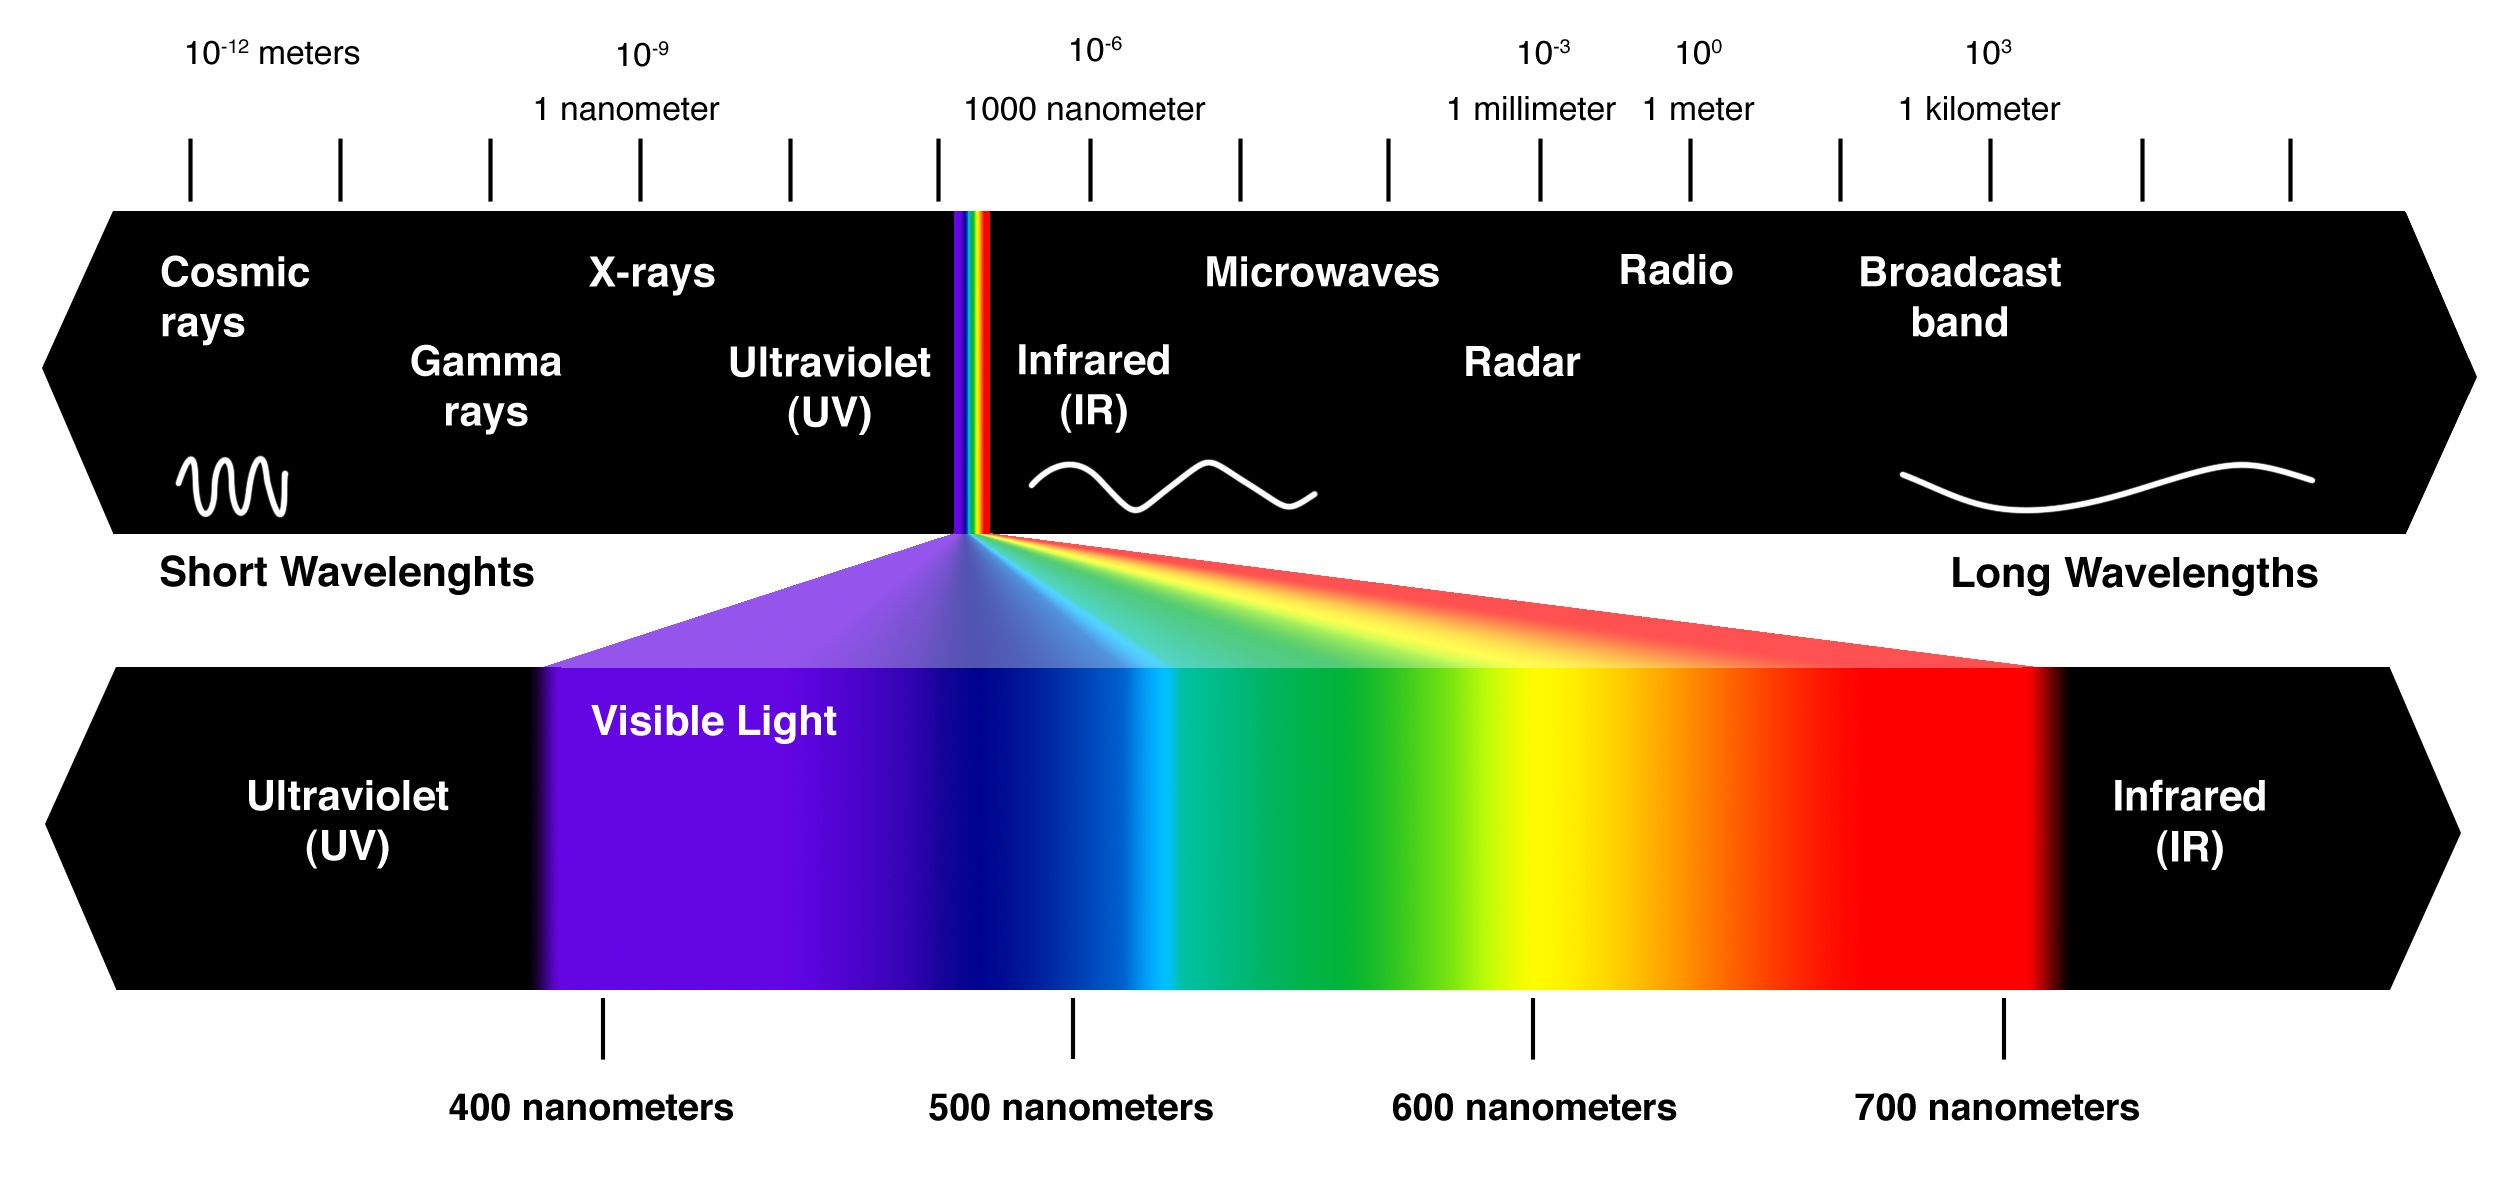
\includegraphics[width=3.5in]{Images/IR Sensor/IR_spectrum.jpg}
	\caption{Infrared Spectrum}
\end{figure}

Based on their range of wave lengths, \ac{IR} can be further classified into three regions. The Near Infrared regions spans from 700nm to 1400nm and is widely used in most of the \ac{IR} sensors and fibre optics. The Mid infrared region spans from 1400nm to 300nm and is mainly used in heat sensing applications. The Far infrared region that spans from 300nm to 1mm is majorly used in thermal imaging. These different region are effectively used to build various application like night vision devices, infrared astronomy, infrared missile tracking etc.

%------------------------------------------------

\section{Types of \ac{IR} sensors}
There are various \ac{IR} sensors available in the market. Based on their configuration, we can classify them as Active \ac{IR} sensors and \ac{PIR} sensor . Active \ac{IR} sensors are those sensor capable of both producing and sensing \ac{IR} signals while \ac{PIR} sensors mainly consist of detectors. Most of the motion detectors make use of \ac{PIR}. The \ac{PIR} detects the \ac{IR} signals caused due to the heat energy transmitted by any object. In this chapter we would focus on Active \ac{IR} sensor.

\section{Active \ac{IR} Sensors}
\par An active \ac{IR} sensor consist of both \ac{IR} transmitter and \ac{IR} receiver. The transmitter transmits the \ac{IR} signals which would strike on an object and would bounce back to the receiver. However not all signals are bounced from the surface of the object. The bouncing of signals depends on the colour and material of the object. The dark colors have the ability to absorb more energy and transmit only a small portion of the received light. Light colors on the other hand, reflects most of the received light signals. It is this change of deflection of light that gives us the perception for colors. Since \ac{IR} sensor is only capable of detecting the presence/absence of \ac{IR} signals, they are employed to detect bright/dark surfaces. An \ac{IR} sensor is not capable of differentiating various colors.

\begin{figure}
	\centering
	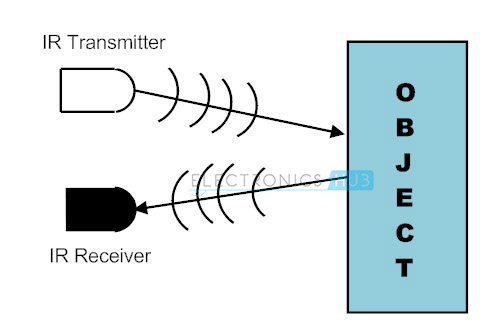
\includegraphics[width=2in]{Images/IR Sensor/IR_wave_bouncing.png}
	\caption{Behaviour of \ac{IR} Sensor}
\end{figure}

\begin{figure}
    \centering
    \subfloat[White surface]{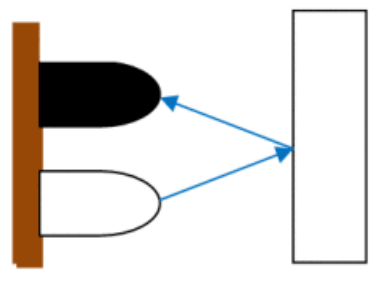
\includegraphics[width=1.5in]{Images/IR Sensor/IR_work_white.png}}\qquad
    \subfloat[Black surface]{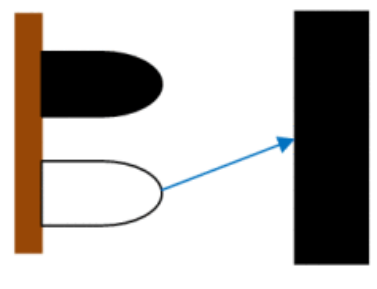
\includegraphics[width=1.5in]{Images/IR Sensor/IR_work_black.png}}
    \caption[]{Working of IR sensor}
\end{figure}

\section{\ac{IR} sensor boards}
Now lets talk about the component required for a complete Active \ac{IR} sensor. An \ac{IR} sensor have two major LED that does the purpose of transmission and detection of signals. A transmission LED looks just like an normal LED diode. Upon applying sufficient voltage across the terminals, the LED produces signals which are transmitted in a straight line. A receiver LED act as an photo-diode that excite electrons upon receiving an \ac{IR} signal. The receiver changes its resistance, which is used to detect the presence of \ac{IR} signal. It is quite easy to identify both the LED. The \ac{IR} receiver would be in dark color to prevent detection of surrounding \ac{IR} signals. Note that the Sun emits a wide range of \ac{EMR}, so it possible for \ac{IR} receiver to detect the \ac{IR} signals from the sunlight. Although it appears just like two LED, we would require proper circuitry to get a calibrated reading. Keep in mind that the receiver and transmitter LED need not always be on the same board, they can have separate circuits to function properly.

\section{Detailing \ac{IR} sensor FC-51}
\par There are various \ac{IR} sensor boards available in the market. You may choose any \ac{IR} sensors suitable for your application. However the underlying principle of \ac{IR} sensor are the same. Here we would make use of \ac{IR} sensor board FC-51 to interface with Arduino.

\begin{figure}
	\centering
	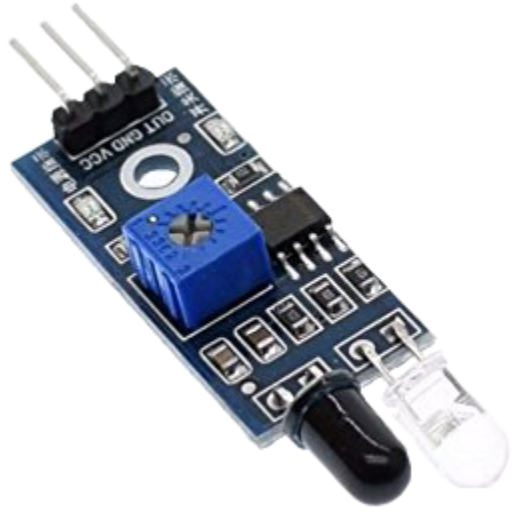
\includegraphics[width=2in]{Images/IR Sensor/IR_board.png}
	\caption{FC-51 IR Sensor board}
\end{figure}

\par A typical \ac{IR} sensor board consist of both the transmitter and receiver diodes along with supporting circuitry which includes a potentiometer, an \ac{IC} and a couple of resistors and LEDs. The potentiometer is used to adjust the sensitivity of the board. The more sensitive the board is, greater will be the amplification of weak signal detected. In other words, it would be able to detect \ac{IR} signal from greater distance. The \ac{IC} would amplify the change in the resistance of \ac{IR} receiver LED and trigger corresponding voltage variations. We can also find two additional indicative LED on the board. One of the LED glows if the board is powered and the other LED glows when the board detects \ac{IR} signals.

\begin{figure}	
	\centering
	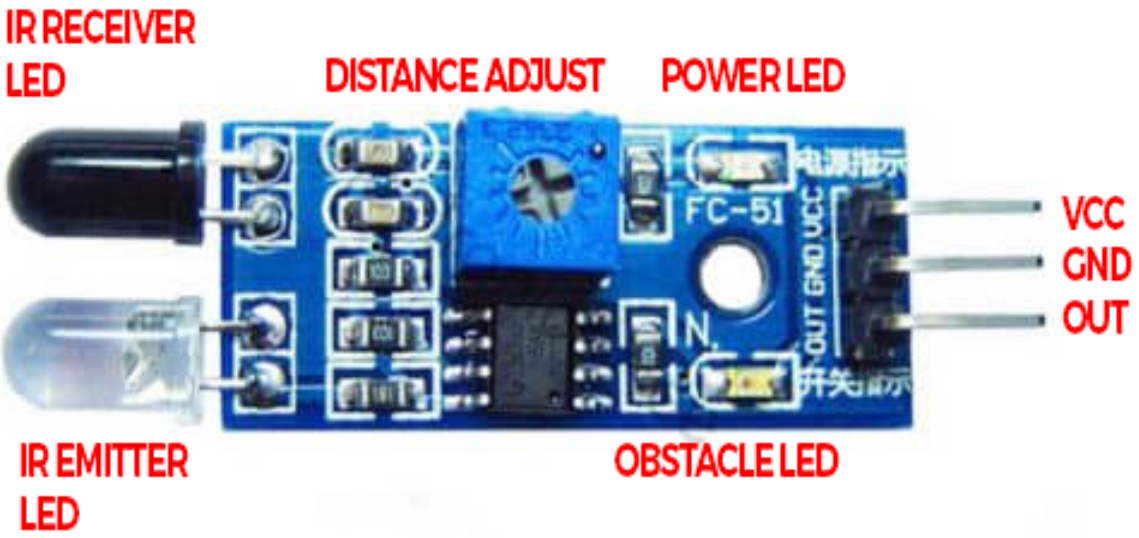
\includegraphics[width=3in]{Images/IR Sensor/IR_board_desp.png}
	\caption{\ac{IR} sensor board description}
	\setfloatalignment{b}
\end{figure}

 Now lets talk about the pins on the board. FC-51 have three legs for interfacing with Arduino. Each legs have there associated marking on the board to indicate what that leg is used for. The VCC pin indicates the power in for the board. The 5v supply from micro-controller is connected to the VCC and the ground (GND) of the board is connected to the GND pin of micro-controller. The OUT pin of the board would act as the input for the Arduino. The OUT pin gives out 5V upon detecting a bright surface and 0V upon detecting a dark surface. There do exist inverted boards that just detects the opposite! ( see table \ref{tab:inverted}) So keep in mind to check board you have before you start coding. 

\begin{table}
    \centering
    \begin{tabular}{|c|c|c|}
    \hline
    \textbf{\hspace{0.4cm}Type of board\hspace{0.4cm}} & \textbf{\hspace{0.4cm} Color of surface\hspace{0.4cm} }& \textbf{\hspace{0.4cm}OUT signal\hspace{0.4cm}} \\
    \hline
    \centering Non inverted & Bright & 5V(high) \\ \cline{2-3} & Dark & 0V(low) \\
    \hline
    \centering Inverted & Bright & 0V(low) \\ \cline{2-3} & Dark & 5V(high) \\
    \hline
    \end{tabular}
    \caption{Inverted and Non-inverted IR boards}
    \label{tab:inverted}
\end{table}

\hspace{0.5cm}
\par Usually in an digital circuit, voltage below 2.3v is regarded as a low signal ( 0v | binary zero) and those above 2.5v as high signal ( 5v | binary 1). There do exist \ac{IR} sensor boards that provide analog output reading. Make sure to understand the configuration of the board before interfacing with Arduino. With that, let start coding. Since FC-51 gives digital output ( HIGH | LOW ) we would be using digital pin of Arduino to interface.

\section{\textbf{Code example 1}}
Objective: Program to print the status of \ac{IR} sensor to Serial monitor

\begin{lstlisting}[style=CStyle]
int IR_pin = 2;    //connect OUT pin of IR to 2nd pin of Arduino

void setup(){

    pinMode(IR_pin,INPUT);    //IR as an input signal
    Serial.begin(9600);       //Baud rate
}

void loop(){
    
    //Reading the digital state of IR_pin
    int state = digitalRead(IR_pin);	
    
    if( state == HIGH){
        Serial.println("Bright surface detected");
    }
    else{
        Serial.println("Dark surface detected");
    }
    
    //Slow down the code so that serial monitor
    // does not flood with characters
    delay(500);
} 
\end{lstlisting}

\begin{figure}	
	\centering
	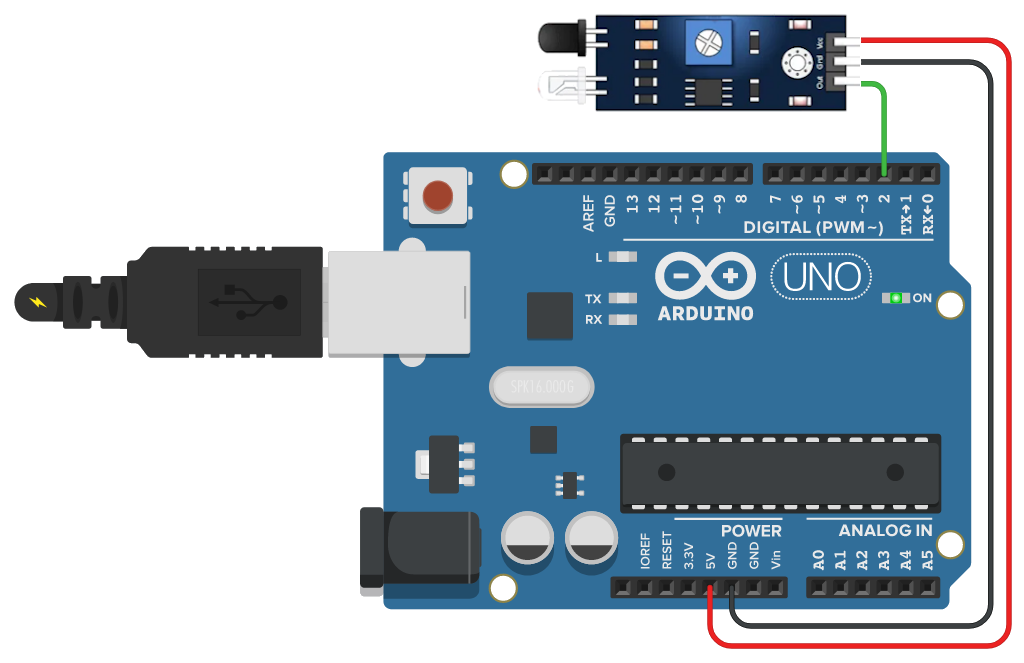
\includegraphics[width=4in]{Images/IR Sensor/circuit1.png}
	\caption{Interfacing \ac{IR} with Arduino}
	\setfloatalignment{b}
\end{figure}

\par Set the serial monitor at 9600 baud rate and see the results. We can find that when there is no object in front of sensor or in the presence of a dark object, the serial monitor shows "Dark surface detected". The monitor would show "Bright surface detected" when there is a white/reflective surface is introduced. Keep in mind that the sun light/flames also emit \ac{IR} radiations that can be detected by \ac{IR} sensors.

\section{\textbf{Code example 2}}
Objective: Program to turn on the in-build LED at pin 13 of Arduino Uno if \ac{IR} sensor detects a while surface. Else keeps the LED off. The circuit of previous example can be used.

\begin{lstlisting}[style=CStyle]
int IR_pin = 2;
int LED = 13;

void setup(){
    pinMode(IR_pin,INPUT);
    pinMode(LED,OUTPUT);
}
void loop(){
    int state = digitalRead(IR_pin);
    digitalWrite(LED, state);
    
    //alternatively use the single line code
    //digitalWrite(LED,digitalRead(IR_pin));
    
    delay(200);
}
\end{lstlisting}


\section{Line Follower bot}

\par Line follower bot is an simple bot that make use of \ac{IR} sensors. The bot consist of \ac{IR} sensors ( usually an \ac{IR} sensor array - figure \ref{fig:ir_array}), wheel and motors, motor driver, Voltage source all placed in a chassis. An \ac{IR} array is a collection of 4 to 6 \ac{IR} sensor receive and transmitter. We would be reading values from individual pair of sensors. Another major component is the motor driver. As the name suggests, they are used to drive motors. Jump to the chapter \ref{chap:Motor_Driver} to setup the bot - wheels and motors.

\begin{marginfigure}	
	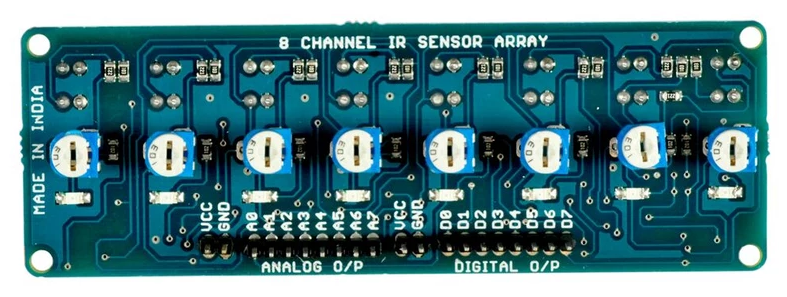
\includegraphics{Images/IR Sensor/IR_array.png}
	\captionsetup{type=figure}
	\caption{\ac{IR} Array}
	\label{fig:ir_array}
\end{marginfigure}

Line follower bot follows a line to its destination. To detect the more precisely, the paths is formed by black lines in a white background or white path in black background. Usually the later is chosen as it is easy to construct black path in white background. For this simple bot, we would be making use of two \ac{IR} sensors instead of an \ac{IR} array. Our bot would have two wheels instead of four, although it is easy to extend to four wheels.

\begin{figure}
    \subfloat[\ac{IR} Bot]{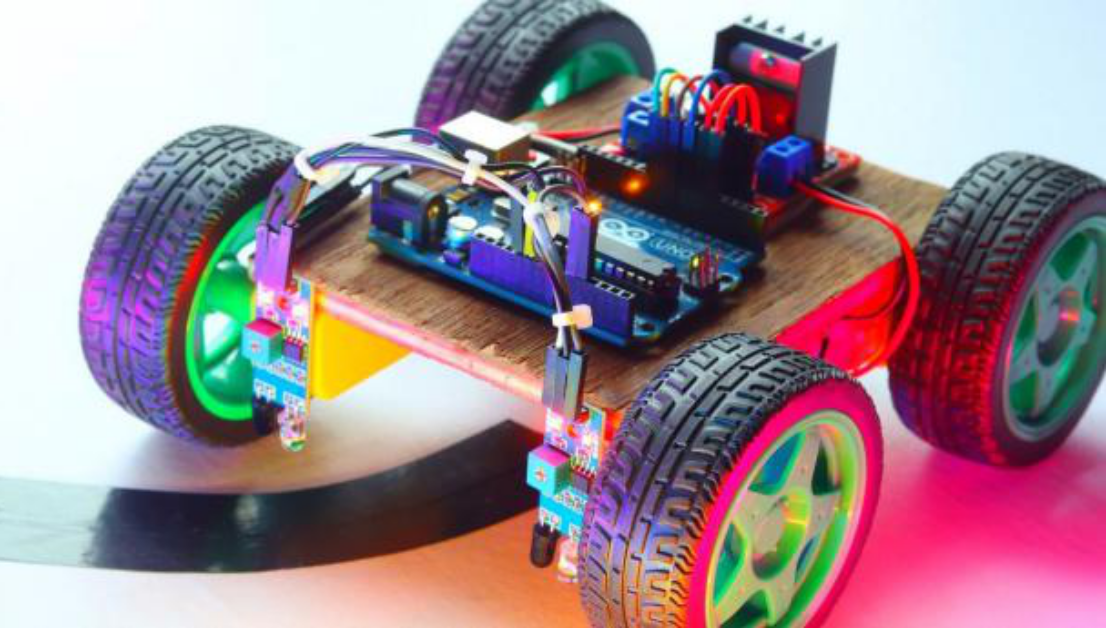
\includegraphics[width=2in]{Images/IR Sensor/line_follower_bot1.png}}
    \quad
    \subfloat[Line follower path]{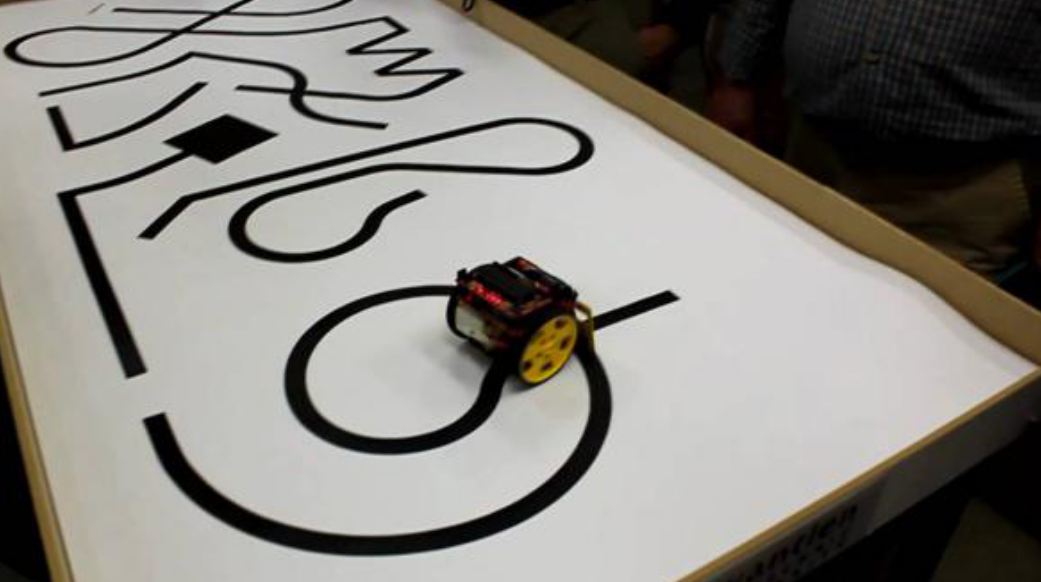
\includegraphics[width=2in]{Images/IR Sensor/line_follower_path.png}}
    \caption{Line follower - bot and path}
\end{figure}

\section{Tracing line - Line follower}

The main event of the line follower is to trace the line. In our sample environment, we would be using two \ac{IR} sensors to detect the black line on the while surface. The bot is placed such that the black line moves right through the center of the bot. Both the sensors are places right next to the dark line.

\begin{marginfigure}
    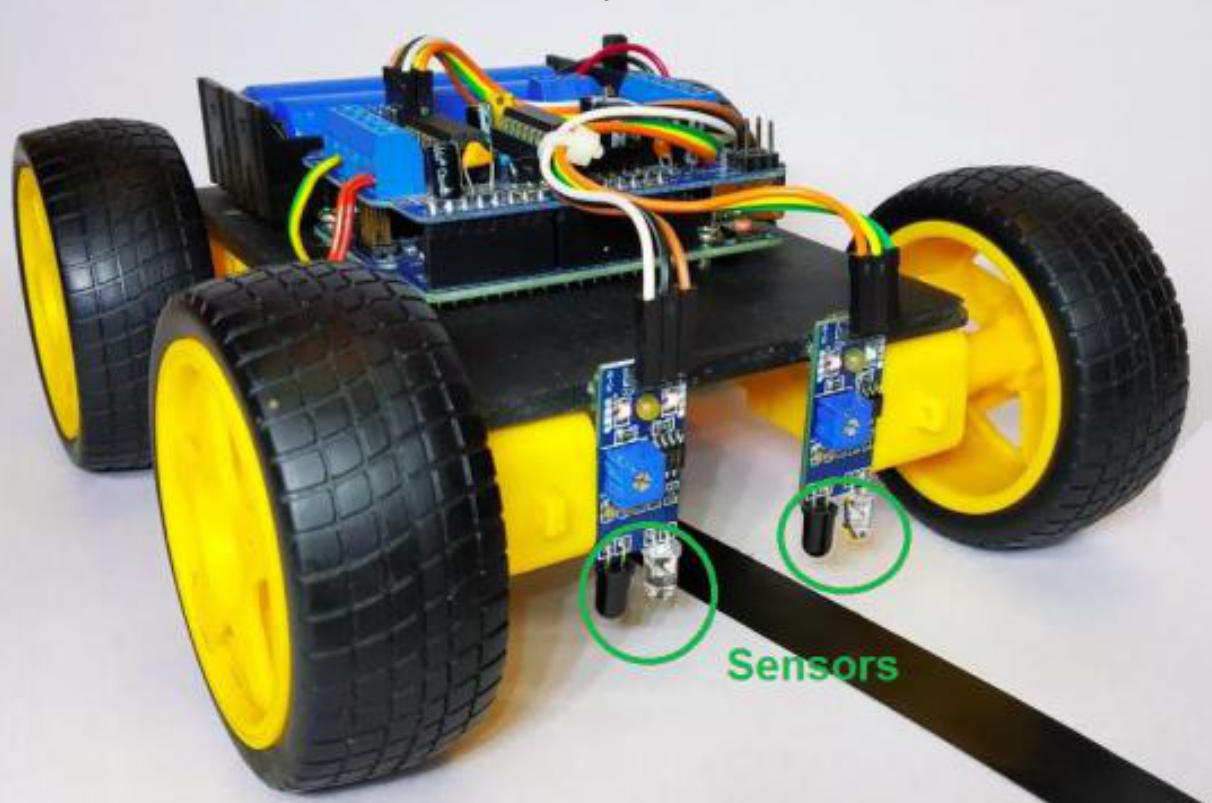
\includegraphics{Images/IR Sensor/sensor_align.png}
    \captionsetup{type=figure}
    \caption[Line Follower Sensor]{ \raggedright Line follower sensor alignment}
\end{marginfigure}

Table \ref{tab:line_follower_move} have listed all sort of possible combinations with 2 \ac{IR} sensors. Now lets implement them in our bot. Take a quick peek at the section \ref{section:bot_interface} where we have programmed a small bot. Lets add the additional \ac{IR} sensors to them to complete our line follower.

\renewcommand{\arraystretch}{3.6}
\begin{table*}
    \centering
    \begin{tabular}{|c|c|c|c|c|}
    \hline
        \textbf{Path property} & \textbf{Left IR} & \textbf{Right IR} & \textbf{Bot Motion} & \textbf{Scenario} \\ \hline
        Straight path & HIGH (white) & HIGH (white) & Forward & \begin{minipage}{.3\textwidth}
            \centering
            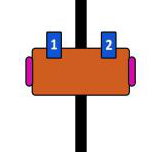
\includegraphics[width=20mm, height=20mm]{Images/IR Sensor/IR_linefollower_straight.png}
            \vspace{1mm}
        \end{minipage} \\ \hline
        Makes a right curve & HIGH (white) & LOW (black) & Turn right & \begin{minipage}{.3\textwidth}
            \centering
            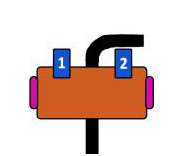
\includegraphics[width=20mm, height=20mm]{Images/IR Sensor/IR_linefollower_right.png}
            \vspace{1mm}
        \end{minipage}  \\ \hline
        Makes a left curve & LOW (black) & HIGH (white) & Turn left & \begin{minipage}{.3\textwidth}
            \centering
            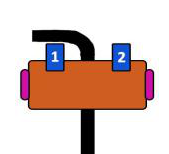
\includegraphics[width=20mm, height=20mm]{Images/IR Sensor/IR_linefollower_left.png}
            \vspace{1mm}
        \end{minipage}  \\ \hline
        Cross bar & LOW (black) & LOW (black) & Stop & \begin{minipage}{.3\textwidth}
            \centering
            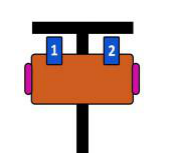
\includegraphics[width=20mm, height=20mm]{Images/IR Sensor/IR_linefollower_stop.png}
            \vspace{1mm}
        \end{minipage}  \\ \hline
    \end{tabular}
    \setfloatalignment{b}
    \vspace{9mm}
    \caption{Line follower movement}
    \label{tab:line_follower_move}
\end{table*}
\renewcommand{\arraystretch}{1}

\begin{figure}
    \centering
    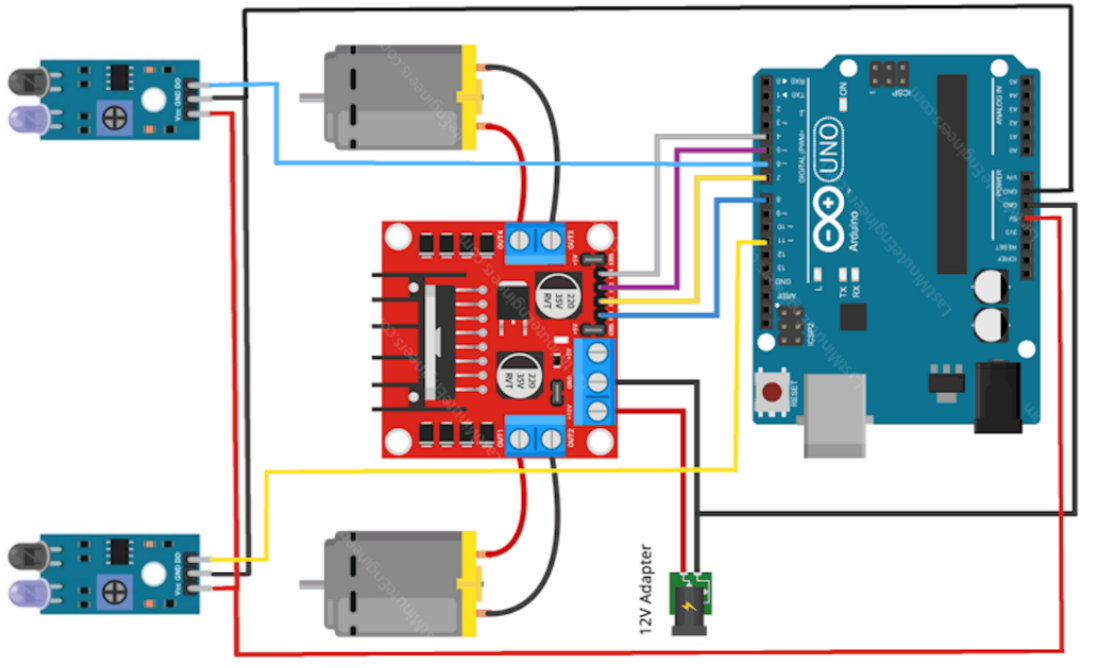
\includegraphics{Images/IR Sensor/ir_bot.png}
     \caption{\ac{IR} Line follower Circuit}
     \label{fig:ir_bot}
\end{figure}

\par Lets detail the connection of the circuit show in figure \ref{fig:ir_bot}. The VCC and GND of \ac{IR} sensors are connected to 5V and GND of Arduino. The left \ac{IR} sensor (bottom) gives its output to 11th pin of Arduino while the right \ac{IR} sensor (top) gives its output to 6th pin of Arduino. The GND of motor driver is connected to the GND of Arduino and input1, input2, input3, input4 of driver are connected to pins 8, 7, 5, 4 pins of Arduino respectively. Left motor is connected to the channel A and right motor is connected to channel B of the motor driver. Finally we powered the driver using a 12v adapter and connected the GND of driver and Arduino to it. Now lets implement the logic depicted on the table \ref{tab:line_follower_move}.

\begin{lstlisting}[style=CStyle]
int m1 = 8, m2 = 7;    //left  motor pins
int m3 = 5, m4 = 4;    //right motor pins
int ir1 = 11, ir2 = 6; //left and right \ac{IR} sensor inputs

void setup(){
    //set motor pins as output for Arduino.
    pinMode(m1,OUTPUT); pinMode(m2,OUTPUT);
    pinMode(m3,OUTPUT); pinMode(m4,OUTPUT);
    
    //set IR pins as input for Arduino
    pinMode(ir1, INPUT); pinMode(ir2, INPUT);
    
    Serial.begin(9600);
}

//A function to control motor movement
void turn_motor(int input1, int input2, char dir){
    if( dir == 'F'){
        //clockwise rotation
        digitalWrite(input1,HIGH);
        digitalWrite(input2,LOW);
    }
    else if( dir == 'S'){
        //no rotation
        digitalWrite(input1,LOW);
        digitalWrite(input2,LOW);
    }
}

void loop(){
    //reading the IR sensors
    int left  = digitalRead(ir1);
    int right = digitalRead(ir2);
    
    if( left == HIGH && right == HIGH){//Forward motion
        turn_motor(m1, m2, 'F');           
        turn_motor(m3, m4, 'F');           
        Serial.println("Bot moving forward");
    }
    else if(left == HIGH && right == LOW){//Right motion
        turn_motor(m1, m2, 'F'); 
        turn_motor(m3, m4, 'S');
        Serial.println("Bot turning right");
    }
    else if(left == LOW && right == HIGH){//Left motion
        turn_motor(m1, m2, 'S');  
        turn_motor(m3, m4, 'F'); 
        Serial.println("Bot turning left");
    }
    else{								//Stopping the bot
        turn_motor(m1, m2, 'S');
        turn_motor(m3, m4, 'S');
        Serial.println("Bot paused");
    }
    delay(100);
}
\end{lstlisting}

\par You might have noticed that the bot drifts or becomes unstable when it changes it direction suddenly. This is because the wheels are rotating with higher speed than our bot can handle. The solution to such problems is the control the speed of the wheels. Refer the section \ref{section:speed_controlled_bot} to build speed controlled bot. You may also find that bot travels in a zig-zag fashion, the curves are not covered smoothly or the bot may miss some sharp curves. To avoid such problems, line followers are build using an \ac{IR} array, where there are more sensors to detect the intensity of curves etc. 

\paragraph{ } Line follower is one of the popular projects in Arduino-ROBOTICS. Various competitions are held across the world with varying difficulty and challenges. Maze solver is one of the most common event held. Speed, accuracy and reliability of bots are noted to announce the winner. To improve the probability of bagging the price, various statistical theories, mathematical models are applied and coded into the programs. Here we have detailed the basics of line follower. The rest is left to you to explore!

\begin{figure}
    \centering
    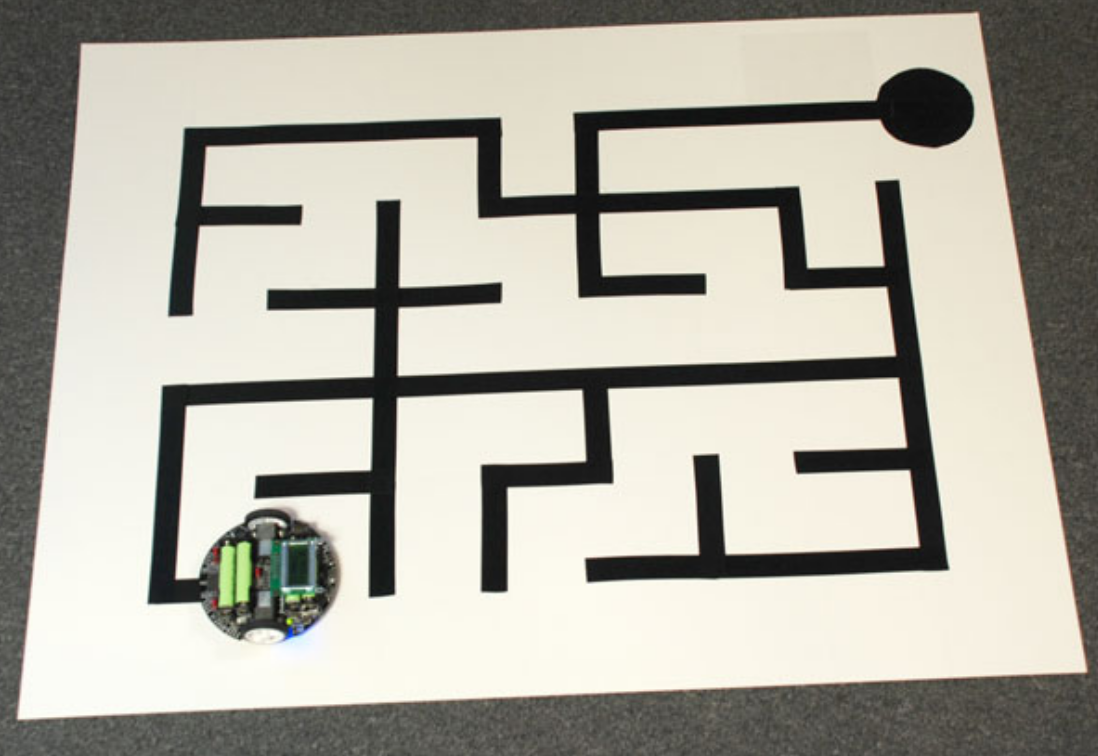
\includegraphics{Images/IR Sensor/line_maze.png}
    \caption{Line follower maze}
\end{figure}